\chapter{Slave controllers}
\label{ch:slave}
Each slave controller directly handles a single dc motor, receiving commands
from the master controller via I2C. It must offer an interface to get and
manipulate its motor's speed.

The slave controller produces a PWM wave having a duty cycle consistent with
the speed (given in RPM) specified by the end user in order to control its
motor.

Furthermore, it comes with a software Proportional-Integral-Derivative
controller to correct the bias between target and actual motor speeds.

\section{Hardware setup}
The slave controller itself is an AVR \emph{ATMega2560} microcontroller
unit\cite{at2560-ref}, which offers the following features of interest:

\begin{itemize}
  \item Dedicated I2C hardware subsystem
  \item PWM-capable 8-bit and 16-bit timers
\end{itemize}

Apart from the motor itself (along with its power supply and its dedicated
H-bridge control board) no additional hardware is used.

\section{I2C setup}
A slave controller communicates with the master controller using the I2C
protocol. As for the master controller, both transmission and reception are
interrupt-based.

The slave controller is always passive on the bus, waiting to be addressed by
the master.

\subsection{Dynamic I2C addressing}
Each slave controller needs a unique I2C address. Basically, there are two ways
to assign an arbitrary address to a slave.

The first and most trivial one is to define the \texttt{TW\_DEFAULT\_ADDR}
macro to the desired address when building the slave controller firmware. This
solution is impractical for obvious reasons and should be avoided.

The second method is to connect the master and slave controllers via I2C and
the master controller with the client via serial. Then the
\texttt{set-slave-addr} command can be used to change the I2C address to the
desired one. The changes take place immediately, as the slave controller's I2C
software module is reinitialized, and they will be saved in the EEPROM embedded
into the AVR microcontroller for durability.

\section{Proportional-Integral-Derivative controller}
An own-written, software-defined Proportional-Integral-Derivative controller is
used to correct the actual motor speed. As for any PID device, the equation
controlling the error is:
\begin{equation}
  u(t) = K_p e(t) + K_i \int_{t_0}^t e(\tau)\,d\tau + K_d \frac{d}{dt}\,e(t)
\end{equation}
being:
\begin{itemize}
  \item $e(t)$ the measured speed error
  \item $u(t)$ the PID control variable
  \item $K_p$ the proportional gain
  \item $K_i$ the integral gain
  \item $K_d$ the derivative gain
\end{itemize}

\subsection{Measuring speed}
For actual PID capabilities, the slave controller must sample the actual speed
of the dc motor at fixed intervals. Therefore, the motor must have an embedded,
two-phase digital encoder.

In fact, one phase is wired to an interrupt-enabled input pin, so the slave
controller is notified immediately when an encoder signal (raising edge) is
generated. Every sampling interval, the PID routine takes the motor's actual
position (measured by the cumulative number of encoder triggers) and computes
its real speed.

\subsection{Approximations}
Of course, a software digital PID controller can not compute exact integrals
and derivatives, so it is necessary to use approximation.

The integral operation is approximated using \emph{Riemann sums}. Given a time
delta $\Delta t$ (the actual speed sampling interval in this particular case),
the approximating law is defined as:
\begin{equation}
  \int_{t_0}^t e(\tau)\,d\tau \approx \sum_{k=1}^n e(t_k^*) \cdot \Delta t
\end{equation}
The derivative operation is approximated using its
definition\cite{levy-num-analysis}:
\begin{equation}
  \frac{d}{dt}\,e(t) = \lim_{\Delta t \to 0} \frac{e(t + \Delta t) - e(t)}{\Delta t} \implies
  \frac{d}{dt}\,e(t) \approx \frac{e(t + \Delta t) - e(t)}{\Delta t}
\end{equation}
being $\Delta t$ a time delta (again, the actual speed sampling interval).

%\subsection{PID parameters}
% TODO

\section{Power management}
The same avr-libc wrapper written for the master controller power management is
used.
By default, the slave controller is in \emph{idle} mode, and it is awakened by
any raised interrupt. The main loop routine is executed and the idle mode is
entered again. Like for the master controller, the slave is put in idle when
waiting for the I2C routines to return.

The AVR idle mode allows the timers to work, so the slave controller can
generate PWM waves to control the motors, even while sleeping.

\section{Specification}

\subsection{Software modules}
An exhaustive list of software modules for the slave controllers firmware is
given in table \ref{tab:slave-spec-modules}. File paths are relative to the
\texttt{slave/} directory.

\begin{table}[ht]
  \begin{tabularx}{\textwidth}{c X X}
    \toprule
    Module & Description & Files \\
    \midrule
    command &
      Interface to handle commands issued by the master controller &
      \texttt{source/command.c},
      \texttt{include/command.h} \\
    dcmotor &
      High-level interface to the dc motor &
      \texttt{source/dcmotor.c},
      \texttt{include/dcmotor.h} \\
    dcmotor\_phy &
      HAL interface for direct (i.e.\ physical) dc motor handling &
      \texttt{source/dcmotor\_phy.c},
      \texttt{include/dcmotor\_phy.h},
      \texttt{include/dcmotor\_phy\_params.h} \\
    dcmotor\_pid &
      PID controller routines &
      \texttt{source/dcmotor\_pid.c},
      \texttt{include/dcmotor\_pid.h} \\
    main &
      Main and power management routines &
      \texttt{source/main.c} \\
    sleep\_util &
      Wrapper for the avr-libc power management facilities &
      \texttt{include/sleep\_util.h} \\
    twi &
      I2C/TWI communication layer &
      \texttt{include/twi.h},
      \texttt{source/twi.c} \\
    \bottomrule
  \end{tabularx}
  \caption{Slave application software modules}
  \label{tab:slave-spec-modules}
\end{table}


\subsection{Modules dependency graph}
The dependency graph for the slave controllers' software modules is shown in
figure \ref{img:slave-deps-graph}. The \emph{debug} module is excluded.
\begin{figure}[ht]
\begin{centering}
  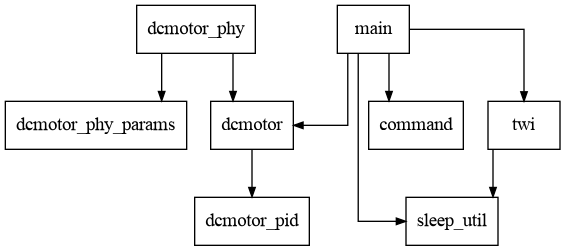
\includegraphics[scale=0.5]{slave-deps}
  \caption{Slave controller modules dependency graph}
  \label{img:slave-deps-graph}
\end{centering}
\end{figure}

\subsection{Circuit schematics}
The complete circuit schematics for the slave controller and all its components
is shown in figure \ref{img:slave-sch}. This circuit can be repeated multiple
times (up to 126) in a single ammc ecosystem.
\begin{figure}[htb]
\begin{centering}
  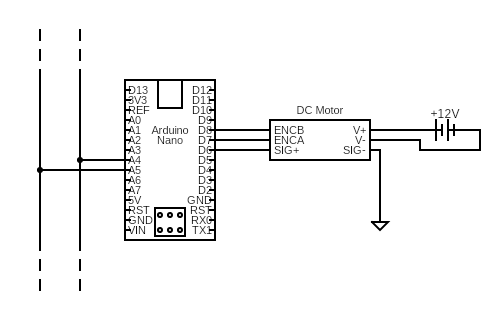
\includegraphics[scale=0.6]{slave-schematics}
  \caption{Slave controller schematics}
  \label{img:slave-sch}
\end{centering}
\end{figure}

\subsection{Wiring}
The wiring correspondence for the slave controller MCU is shown in table
\ref{tab:slave-wiring}.
\begin{table}[htb]
  \begin{tabularx}{\textwidth}{c l X}
    \toprule
    Board pin & MCU pin & Description \\
    \midrule
    D20 & 44/PD1/SDA    & I2C data bus \\
    D21 & 43/PD0/SCL    & I2C clock bus \\
    D13 & 26/PB7        & PWM output to the motor driver \\
    D12 & 25/PB6        & Motor driver direction logic 1 \\
    D11 & 24/PB5        & Motor driver direction logic 2 \\
    D52 & 20/PB1/PCINT1 & Encoder phase B \\
    D53 & 19/PB0/PCINT0 & Encoder phase A, interrupt-enabled \\
    \bottomrule
  \end{tabularx}
  \caption{Slave controller wiring}
  \label{tab:slave-wiring}
\end{table}
